\SubProblem
{مزایا و معایب \lr{CDMA}}
{
در سوال سوم تمرین اول به مقایسه دو روش
\lr{TDMA}
و
\lr{FDMA}
و مزایا و معایب هر یک پرداختیم.
اکنون روش
\lr{CDMA}
را مورد بررسی قرار می‌دهیم و نکات قوت و ضعف آن را ذکر می‌کنیم.

\lr{Code Division Multiple Access}
یا
\lr{CDMA}
روشی برای حل مشکل دسترسی چندگانه است که با اختصاص دادن یک کد به هر کاربر اجازه دسترسی به منابع کانال را می‌دهد.
کدهای ایجاد شده منحصر به فرد هستند و کد هر کاربر با کاربر دیگر متعامد هستند.
در این روش همزمان چندین سیگنال از طریق یک سیگنال با فرکانس ثابت منتقل می‌شوند.

\begin{figure}[H]
    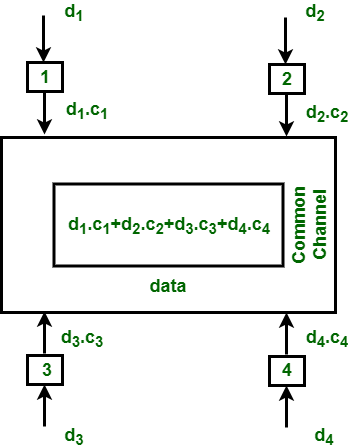
\includegraphics[width=6cm]{Images/CDMA.png}
    \centering
    \caption{\lr{CDMA}}
\end{figure}

از ویژگی‌ها، نکات مثبت و منفی این روش می‌توان موارد زیر را ذکر کرد:

\begin{itemize}
    \item
    در سیستم تلفن همراه فرکانس بالا مورد استفاده است.
    
    \item
    نیازمند اختصاص کدهای متعامد به کاربران است.
    
    \item[+]
    هم زمان و هم پهنای باند میان کاربران به صورت همزمان به اشتراک گذاشته می‌شود.
    
    \item[-]
    همزمان به دو محافظ زمانی و فرکانسی نیاز داریم.
    
    \item[+]
    همگام سازی لازم نیست.
    
    \item[+]
    نرخ انتقال داده در آن زیاد است.
    
    \item[+]
    اطلاعات به صورت دیجیتال منتقل می‌شود.
    
    \item[+]
    در مقایسه با دو روش دیگر بسیار انعطاف پذیر است.
    
    \item[-]
    با افزوده شدن تعداد کاربرها کیفیت کلی سیستم کاهش می یابد.
    
    \item[-]
    نیازمند محاسبات زیاد برای تولید کدهای متعامد است.
    
    \item[-]
    توان مصرفی بالایی دارد.
\end{itemize}
}